\newpage

\chapter{Sprint 4: Alert Management and Energy Consumption Monitoring}

\cfoot{\thepage}

\parindent=0.5in
\onehalfspacing

\section{Introduction}

Sprint 4, titled "Alert Management and Energy Consumption Monitoring," introduces two essential operational subsystems addressing proactive network management and energy efficiency optimization. This sprint addresses user stories US-010 (Alert System), US-011A (Energy Recording), and US-011B (Energy Analytics) from Chapter 2's product backlog.

The Alert Management System provides real-time notification capabilities for network anomalies and equipment failures with intelligent severity classification. The system leverages Supabase real-time subscriptions enabling sub-200ms notification delivery, supporting both automated alert generation from equipment status changes established in Sprint 2 and manual alert creation by operations staff.

The Energy Consumption Monitoring System enables comprehensive tracking and analysis of power consumption across telecommunications sites with automatic cost calculation, visual analytics through interactive charts, and threshold-based alerting for abnormal consumption patterns. Both systems integrate seamlessly with the site and equipment foundations from Sprints 1 and 2, maintaining consistent role-based access control established in Chapter 3.

\section{Sprint Backlog}

During sprint planning, we defined the tasks required for Sprint 4 implementation. Table 6.1 presents the sprint backlog with user stories, tasks, complexity assessments, and effort estimates.

\begin{table}[H]
\centering
\small
\begin{tabular}{|p{2.5cm}|p{4cm}|p{3.2cm}|p{2.2cm}|p{1.5cm}|}
\hline
\textbf{Functionality} & \textbf{User Story} & \textbf{Tasks} & \textbf{Complexity} & \textbf{Estimate} \\
\hline

\multirow{3}{2.5cm}{Auto-Create Alerts (US-010)} & 
\multirow{3}{4cm}{As system, I want to automatically create alerts when equipment faults are detected}
& Equipment monitoring logic & Hard & 5h \\
\cline{3-5}
& & Trigger alert creation & Medium & 3h \\
\cline{3-5}
& & Severity classification & Medium & 2h \\
\hline

\multirow{3}{2.5cm}{Acknowledge Alerts} & 
\multirow{3}{4cm}{As manager, I want to acknowledge critical alerts to track response time}
& Status transition logic & Easy & 2h \\
\cline{3-5}
& & Timestamp capture & Easy & 1h \\
\cline{3-5}
& & Response time calculation & Medium & 2h \\
\hline

\multirow{3}{2.5cm}{Resolve Alerts} & 
\multirow{3}{4cm}{As engineer, I want to resolve alerts after fixing issues}
& Resolution workflow & Easy & 2h \\
\cline{3-5}
& & Status update interface & Easy & 1h \\
\cline{3-5}
& & Completion tracking & Easy & 1h \\
\hline

\multirow{3}{2.5cm}{Real-time Notifications} & 
\multirow{3}{4cm}{As user, I want real-time notifications for critical alerts}
& WebSocket setup & Hard & 4h \\
\cline{3-5}
& & Toast notification UI & Medium & 3h \\
\cline{3-5}
& & Auto-dismiss logic & Easy & 1h \\
\hline

\multirow{3}{2.5cm}{Record Energy (US-011A)} & 
\multirow{3}{4cm}{As manager, I want to record energy consumption data for each site}
& Data entry form & Medium & 2h \\
\cline{3-5}
& & Validation logic & Medium & 2h \\
\cline{3-5}
& & Database insertion & Easy & 1h \\
\hline

\multirow{3}{2.5cm}{View Trends (US-011B)} & 
\multirow{3}{4cm}{As engineer, I want to view energy consumption trends with charts}
& Chart component & Medium & 3h \\
\cline{3-5}
& & Data aggregation & Medium & 2h \\
\cline{3-5}
& & Time period filtering & Easy & 1h \\
\hline

\multirow{3}{2.5cm}{Calculate Costs} & 
\multirow{3}{4cm}{As manager, I want to calculate energy costs automatically}
& Cost calculation engine & Medium & 2h \\
\cline{3-5}
& & Rate configuration & Easy & 1h \\
\cline{3-5}
& & Manual override option & Easy & 2h \\
\hline

\multirow{3}{2.5cm}{Track Patterns (US-011B)} & 
\multirow{3}{4cm}{As admin, I want to track consumption per day and identify patterns}
& Pattern analysis logic & Hard & 4h \\
\cline{3-5}
& & Threshold detection & Medium & 3h \\
\cline{3-5}
& & Alert generation & Medium & 2h \\
\hline

\end{tabular}
\caption{Sprint 4 Backlog with Task Breakdown}
\label{tab:sprint4_backlog}
\end{table}

The backlog totals 52 hours across eight major functionalities. WebSocket implementation complexity stems from real-time bidirectional communication requirements. Pattern analysis requires sophisticated aggregation logic processing historical consumption data.

\section{Conceptual Design}

This section presents the conceptual design models guiding Sprint 4 implementation.

\subsection{Class Diagram}

Figure 6.1 presents the class diagram introducing Alert and EnergyConsumption entities integrating with existing system architecture from Sprints 1 and 2.

\begin{figure}[H]
    \centering
    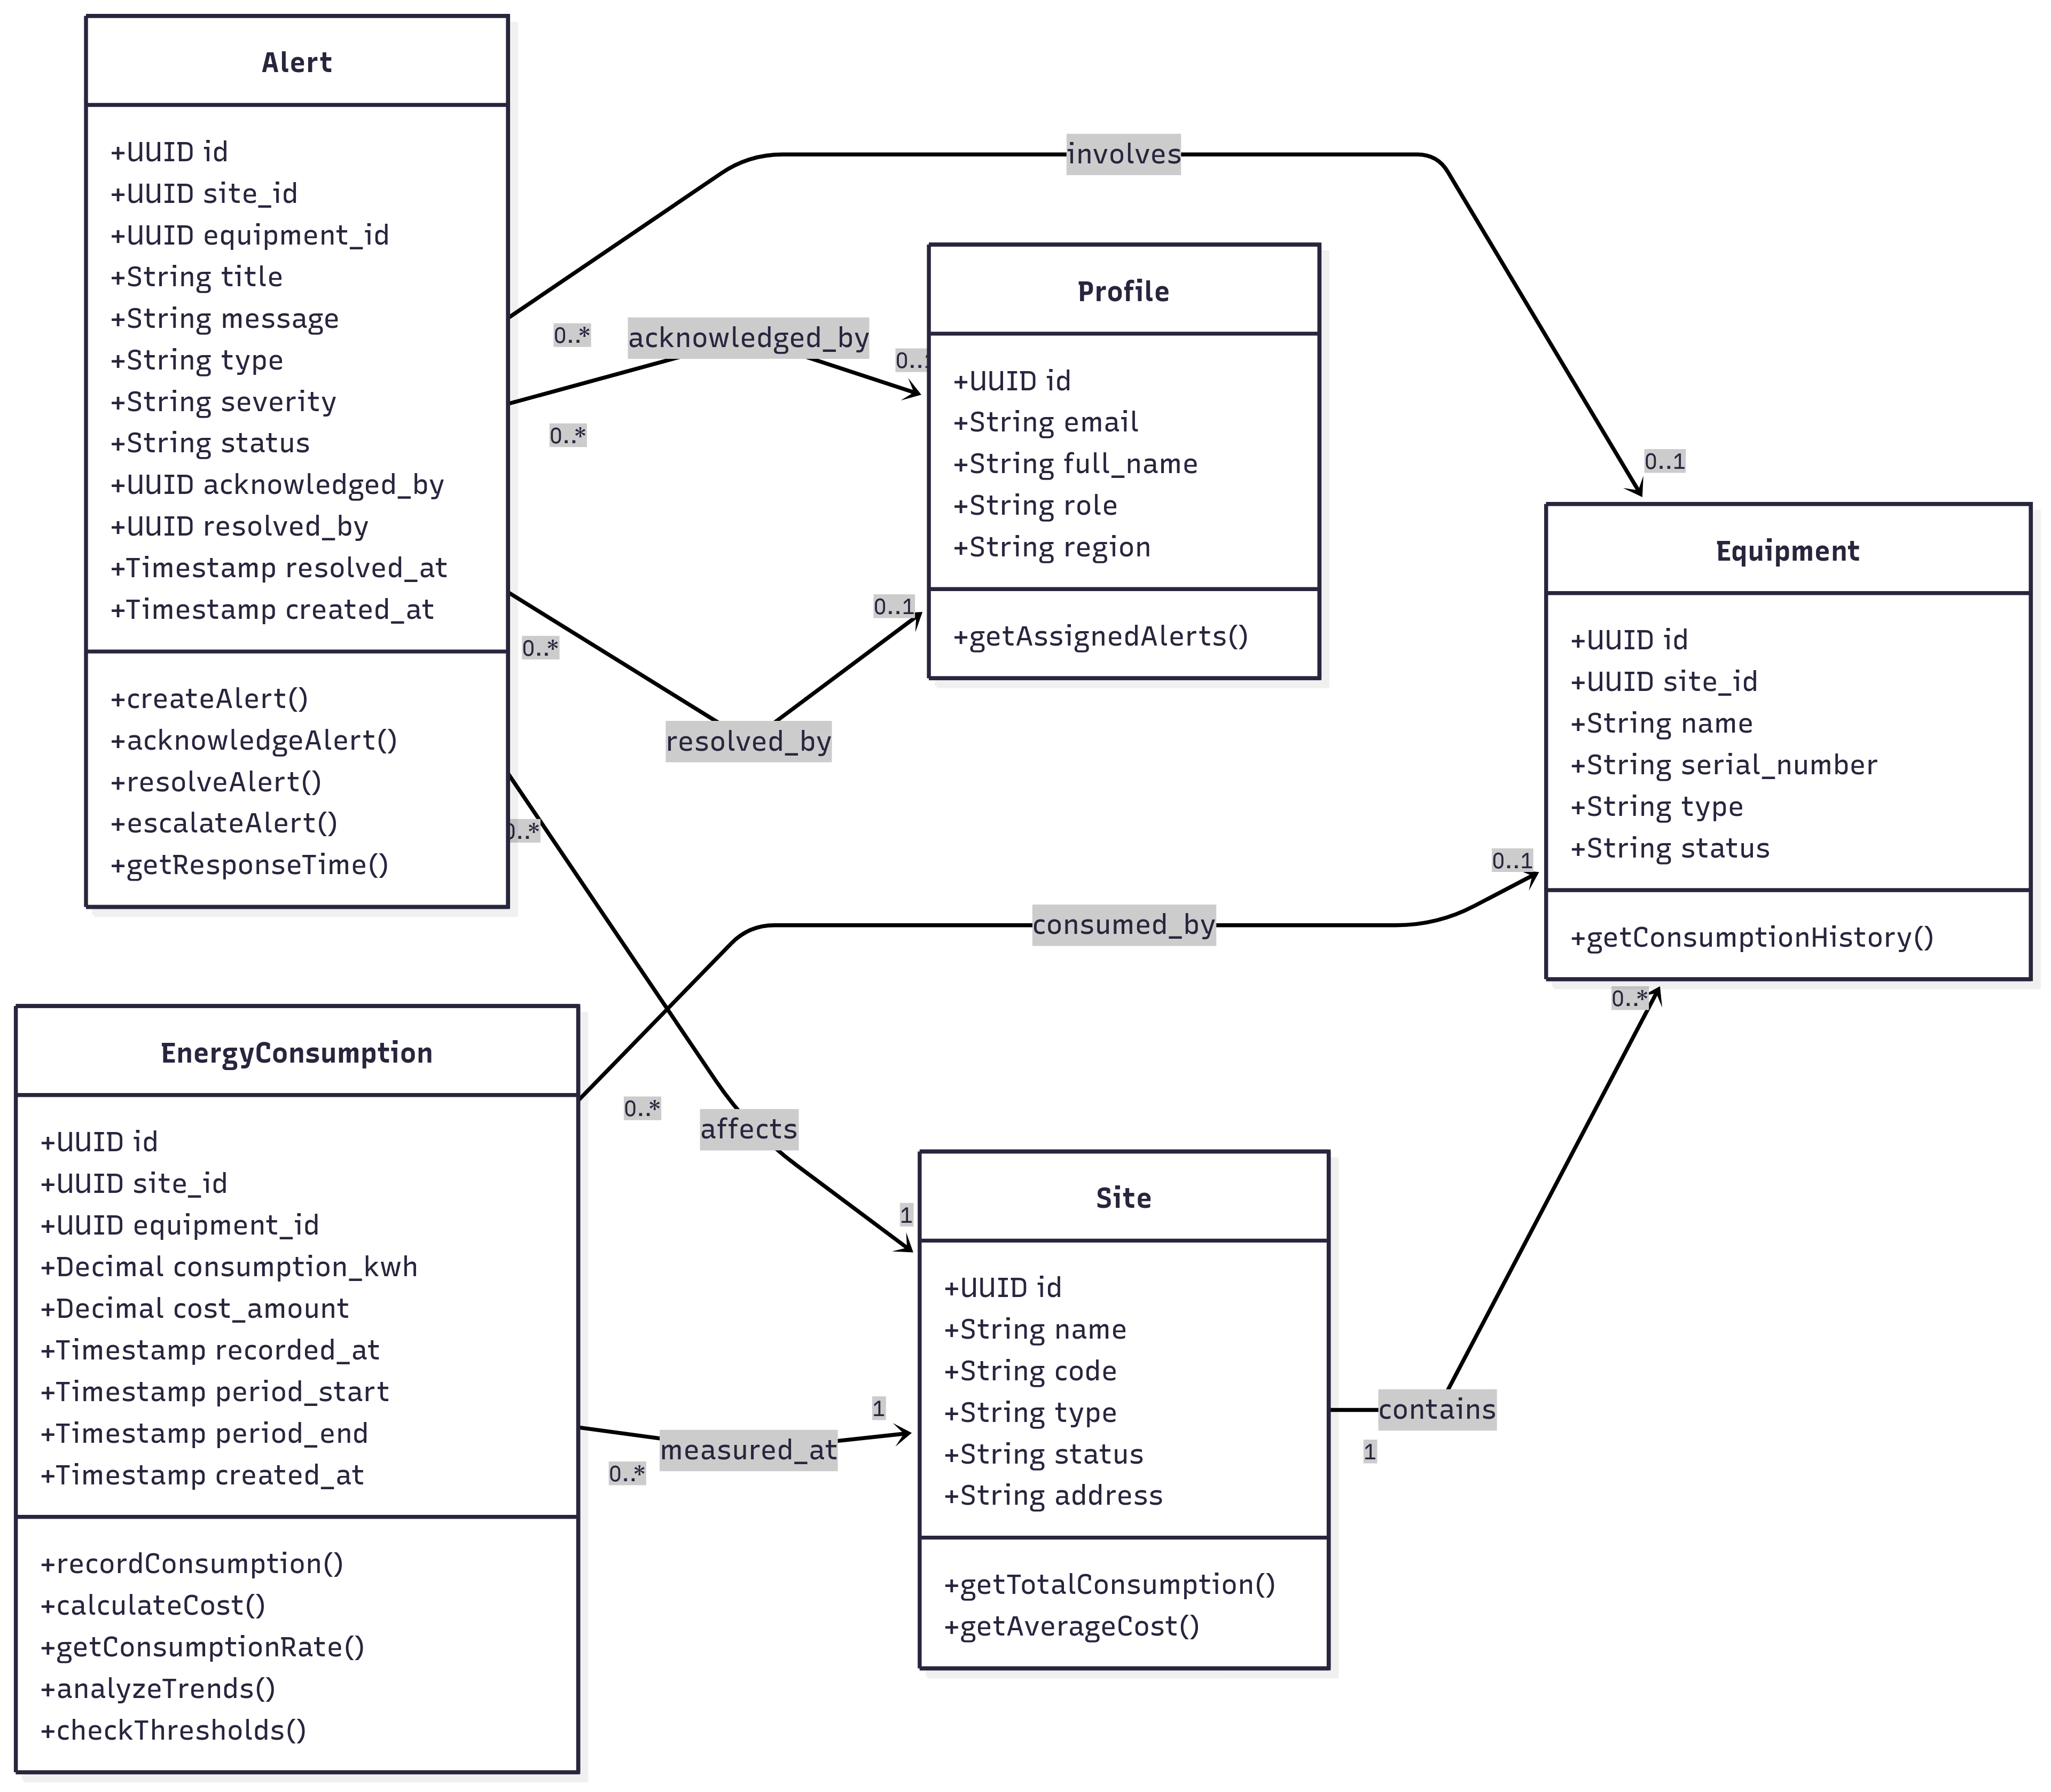
\includegraphics[width=0.95\linewidth]{img/chap_06/class_diagram_sprint4.png}
    \caption{Class Diagram - Alert and Energy Consumption Management}
    \label{fig:class_diagram_sprint4}
\end{figure}

The class diagram (Figure 6.1) illustrates two primary entities using UML standard notation (name : type format). The Alert class manages system notifications with attributes including alert title and message providing notification content, alert type classification (equipment failure, maintenance due, threshold exceeded, system error), severity levels (info, warning, critical) determining escalation procedures, and status workflow (active, acknowledged, resolved) tracking alert lifecycle.

The class implements methods for alert creation with automatic severity assignment, acknowledgment tracking with timestamp capture, resolution marking with completion details, and escalation logic for overdue critical alerts.

The EnergyConsumption class captures power usage data with attributes including consumption value in kilowatt-hours (kWh), calculated cost in Tunisian Dinars based on configurable rates, recording period with start and end timestamps, daily consumption rate calculated automatically, and threshold violation flags. The class supports recording operations with validation, automatic cost calculation, consumption rate analysis, and threshold validation generating alerts for abnormal patterns.

Both entities maintain associations with Site and Equipment entities from Sprints 1 and 2, ensuring proper integration with network infrastructure.

\subsection{Use Case Diagram}

Figure 6.2 presents the use case diagram showing role-based permissions for alert and energy management functionality, following the inheritance hierarchy established in Chapter 3.

\begin{figure}[H]
    \centering
    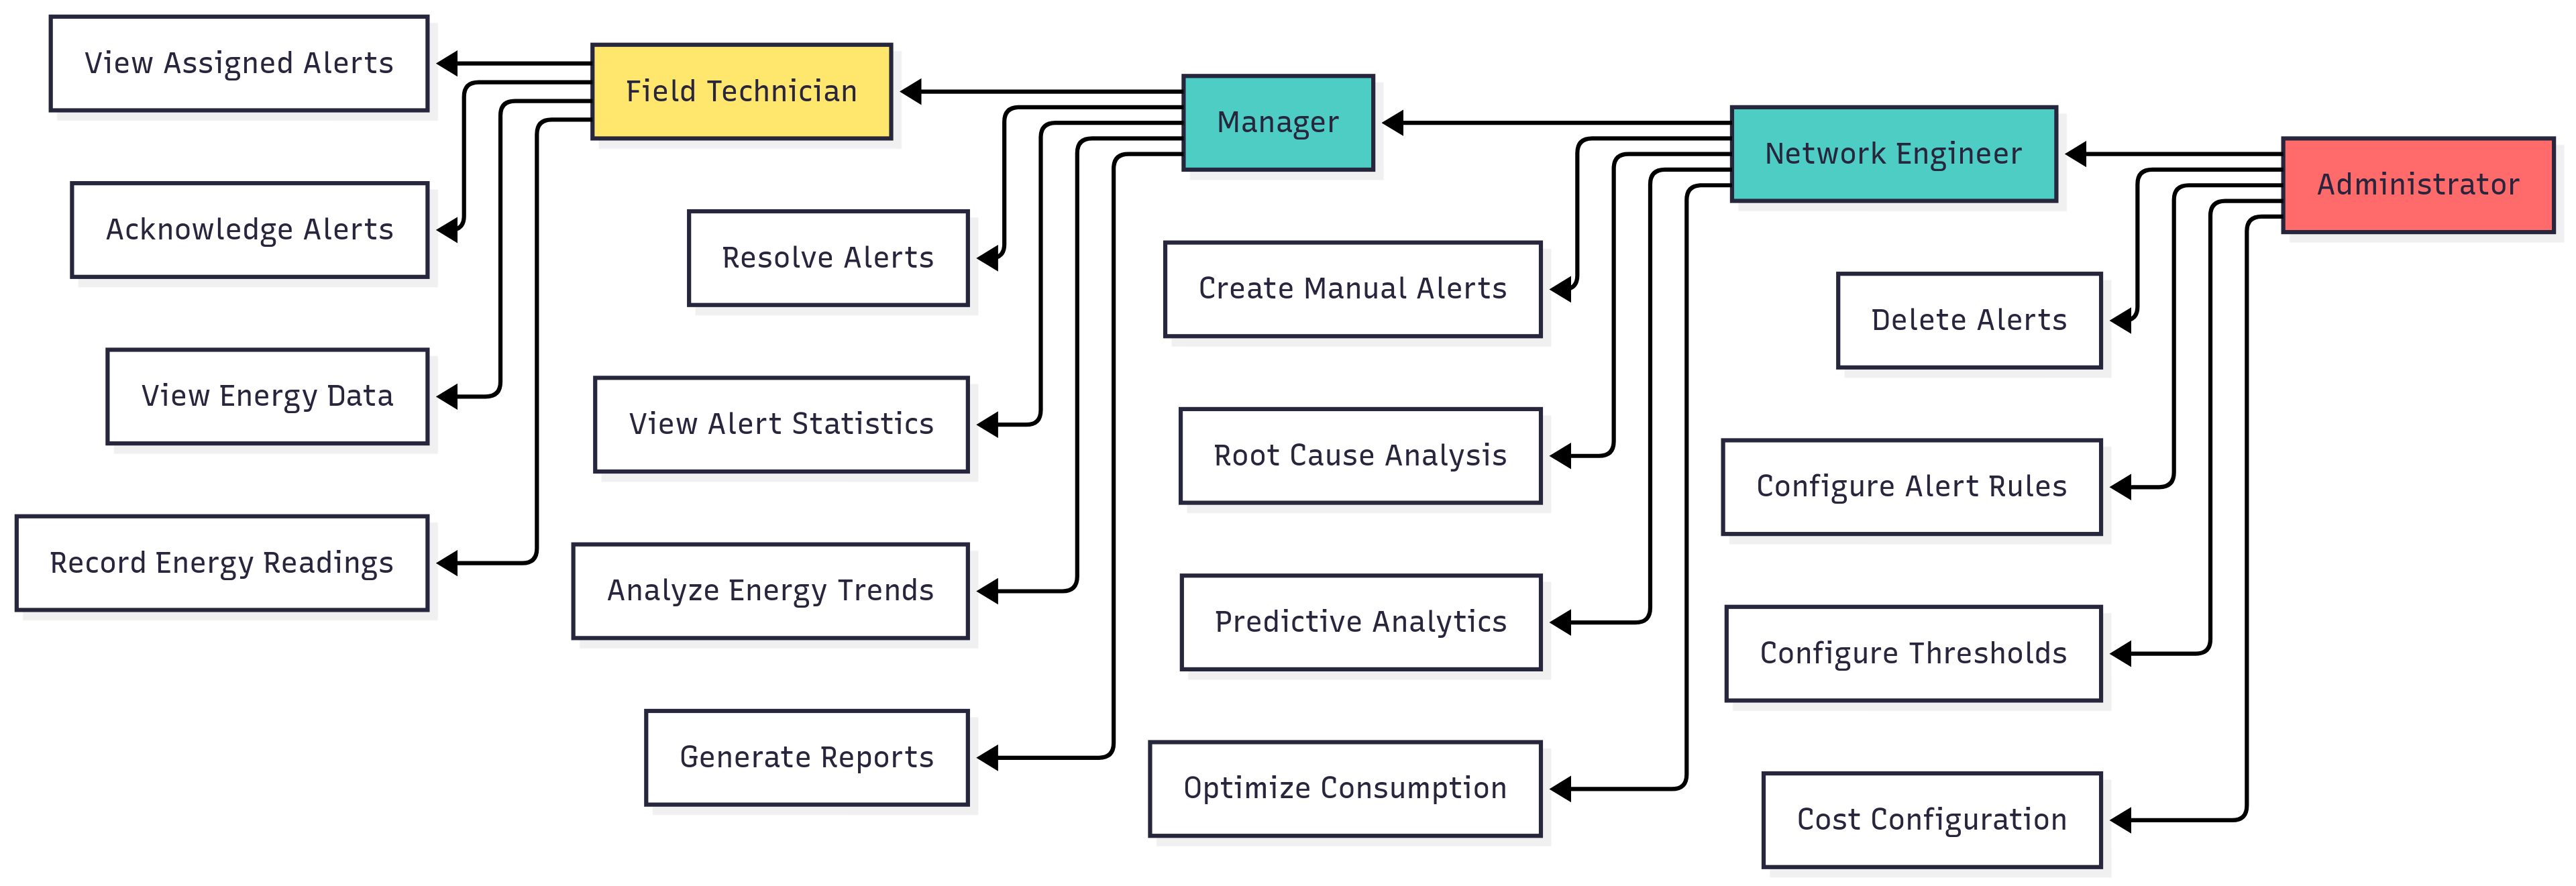
\includegraphics[width=0.45²\linewidth]{img/chap_06/usecase_diagram_sprint4.png}
    \caption{Use Case Diagram - Sprint 4 with Role Inheritance}
    \label{fig:use_case_diagram_sprint4}
\end{figure}

The use case diagram (Figure 6.2) demonstrates the established role inheritance hierarchy from previous sprints. Field Technicians possess base operational capabilities including viewing assigned alerts, acknowledging alerts, viewing energy data, and recording energy readings after site visits.

Managers inherit all technician capabilities while adding supervisory functions including resolving alerts after problem verification, creating manual alerts for observed issues, analyzing energy trends for operational planning, and generating consumption reports for stakeholder communication.

Network Engineers inherit all manager capabilities while adding technical analysis functions including conducting predictive analytics forecasting future consumption patterns and performing advanced trend analysis identifying optimization opportunities.

Administrators inherit all engineer capabilities while possessing exclusive system management rights including deleting alerts for data lifecycle management, configuring alert rules defining automatic generation criteria, configuring consumption thresholds establishing acceptable ranges, and managing system-wide parameters.

\textbf{Use Case Description: Create Alert}

Since alert and energy operations share similar patterns, we provide detailed information on the "Create Alert" use case as representative of Sprint 4 functionality. Table 6.2 presents the detailed textual description.

\begin{table}[H]
\centering
\small
\begin{tabular}{|p{3cm}|p{8.5cm}|}
\hline
\textbf{Element} & \textbf{Description} \\
\hline
\textbf{Use Case Name} & Create System Alert \\
\hline
\textbf{Primary Actors} & Network Engineer, Operations Manager, Administrator \\
\hline
\textbf{Description} & Allows authorized users to manually create alerts for observed issues or proactive notifications \\
\hline
\textbf{Pre-condition} & User authenticated with manager, engineer, or administrator role; Active sites exist; Equipment data available \\
\hline
\textbf{Post-condition} & Alert record created with "active" status; Real-time notifications delivered; System audit log created \\
\hline
\textbf{Main Scenario} & 
1. User clicks "Create Alert" button
2. System displays alert creation form
3. User enters descriptive title
4. User enters detailed message
5. User selects alert type
6. User selects severity level
7. User selects affected site
8. User optionally selects equipment
9. User submits form
10. System validates required fields
11. System creates alert with timestamp
12. System triggers real-time notifications
13. System displays success confirmation
\\
\hline
\textbf{Alternative Flows} & 
A1 - Critical Severity: If severity is "critical", system broadcasts notifications to all managers via WebSocket
A2 - Equipment Association: System dynamically loads equipment list for selected site
A3 - Validation Failure: Display field-specific errors and return to form
\\
\hline
\textbf{Exception Scenarios} & 
E1: Missing required fields → Display validation errors
E2: Invalid data format → Display format error
E3: Server connection failure → Display connection error with retry
E4: Permission denied → Display access denied message
\\
\hline
\end{tabular}
\caption{Detailed Use Case Description - Create Alert}
\label{tab:create_alert_usecase}
\end{table}

\section{Sequence Diagrams}

This section presents sequence diagrams detailing the main processes implemented in Sprint 4.

\subsection{Create Alert Process}

Figure 6.3 demonstrates the complete workflow for manually creating system alerts with real-time notification delivery.

\begin{figure}[H]
    \centering
    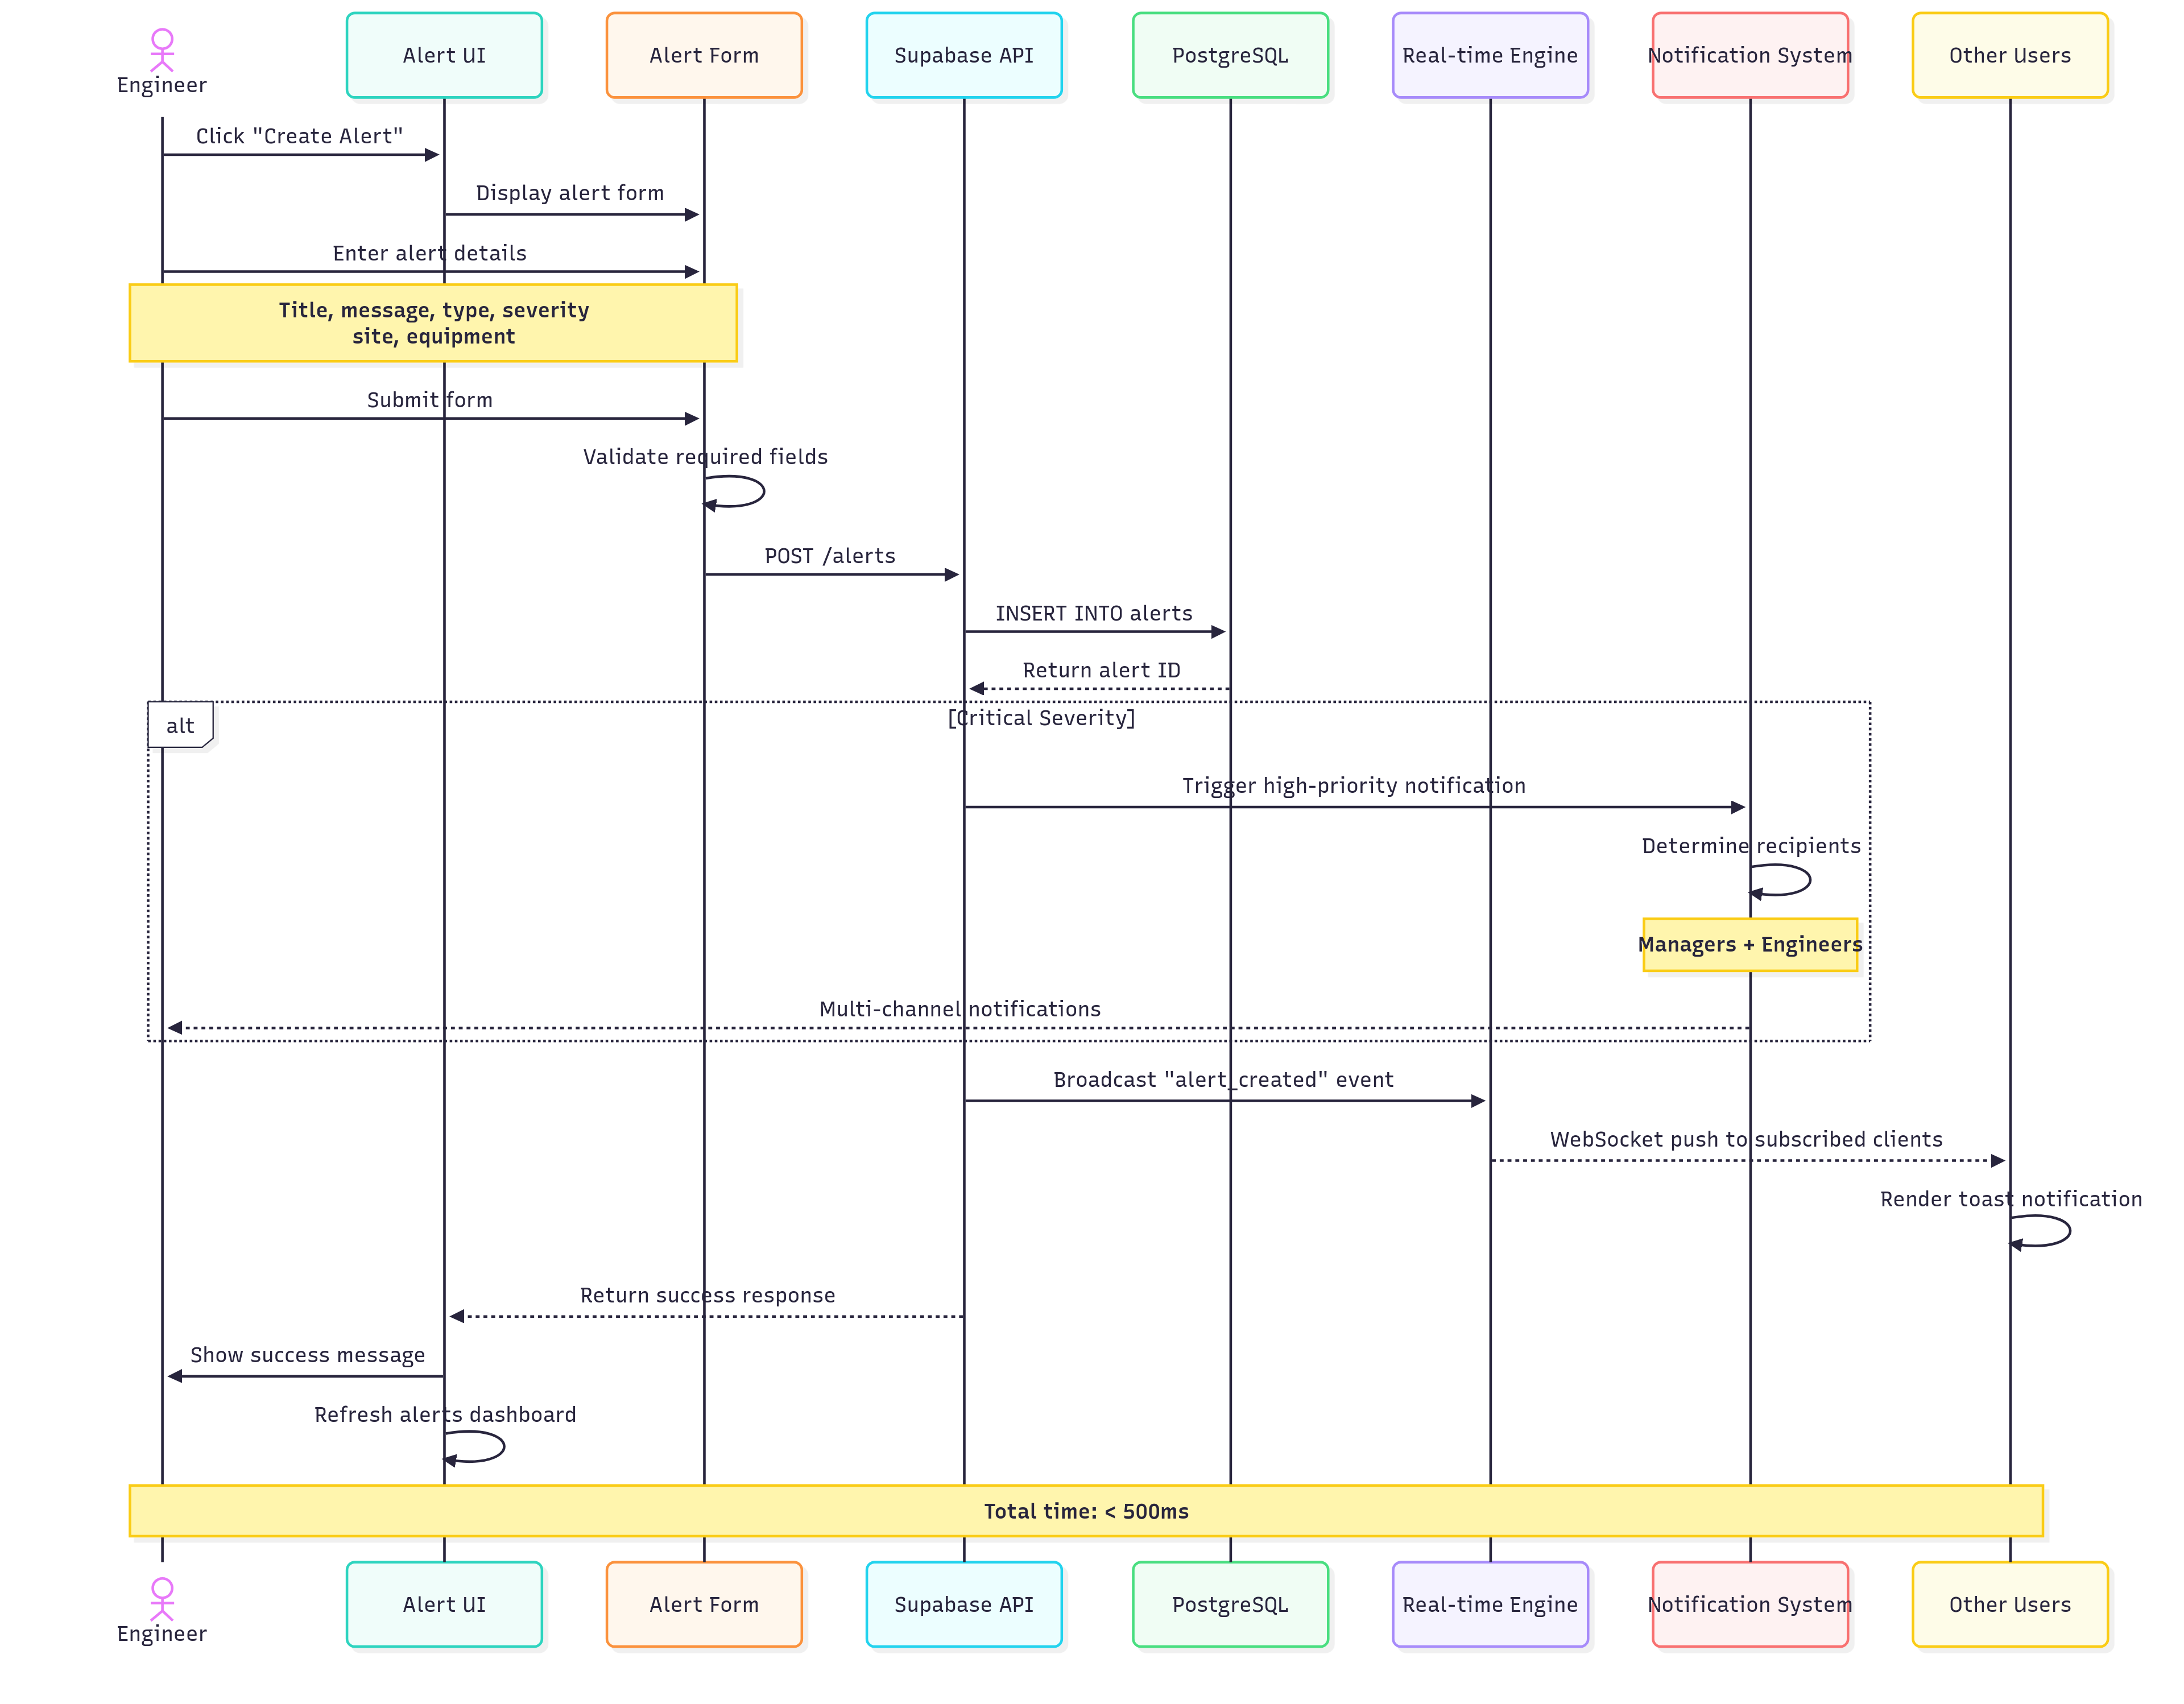
\includegraphics[width=0.95\linewidth]{img/chap_06/sequence_create_alert.png}
    \caption{Sequence Diagram - Create Alert Process}
    \label{fig:sequence_create_alert}
\end{figure}

\textbf{Note on Sequence Diagram:} Following UML sequence diagram standards, return messages should use dashed arrows (-->) while request messages use solid arrows (->), clearly distinguishing between calls and responses.

The create alert sequence (Figure 6.3) demonstrates the workflow for manual alert creation with real-time delivery. An authorized user accesses the alert management interface and clicks "Create Alert" displaying the creation form. The user provides alert information including descriptive title, detailed message explaining context, alert type selection, severity level assignment, affected site selection, and optional equipment association.

Upon form submission, client-side validation ensures required fields are completed. Valid submissions proceed to Supabase via \texttt{supabase.from('alerts').insert()} with Row Level Security verification. The database creates the alert record with "active" status and auto-captured timestamp.

For critical severity alerts, the system triggers the Real-time Engine broadcasting WebSocket events to all subscribed manager sessions. The AlertNotificationToast component renders on recipient screens with slide-in animation, displays alert details with severity-based color coding, provides action buttons for acknowledgment, and auto-dismisses after 10 seconds.

\subsection{Record Energy Consumption Process}

Figure 6.4 illustrates the workflow for recording site energy consumption with automatic cost calculation and threshold validation.

\begin{figure}[H]
    \centering
    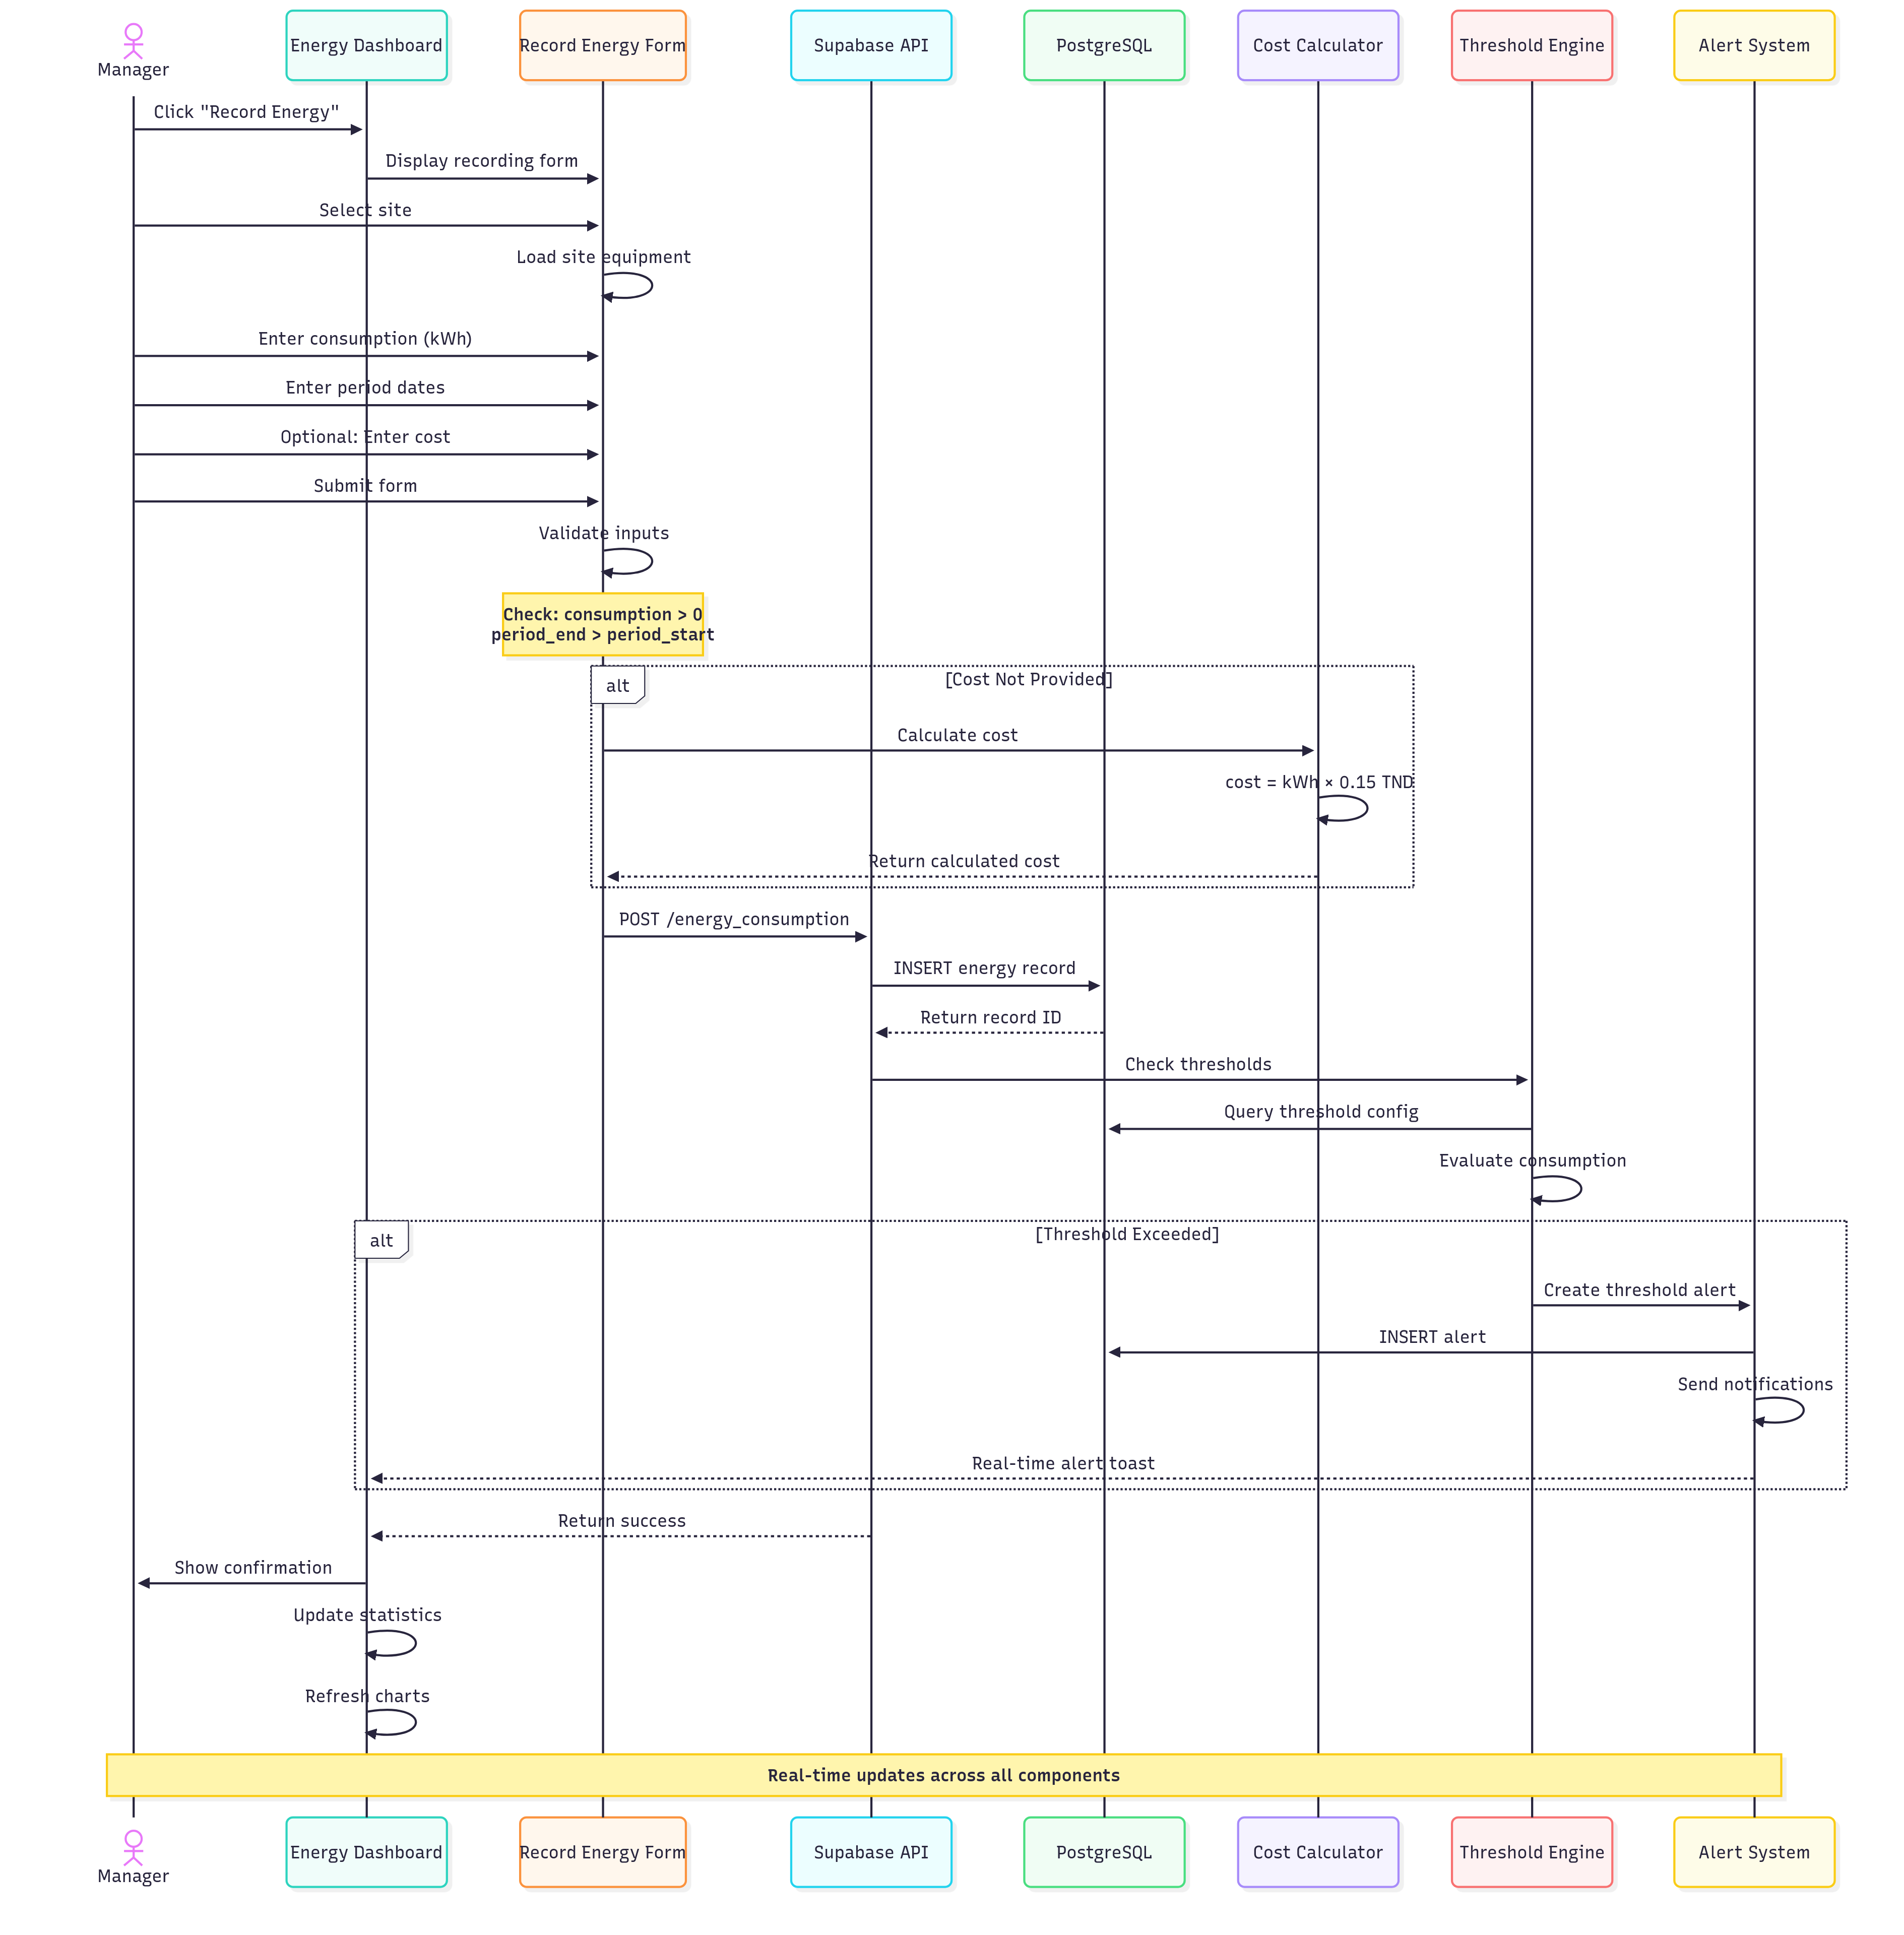
\includegraphics[width=0.95\linewidth]{img/chap_06/sequence_record_energy.png}
    \caption{Sequence Diagram - Record Energy Consumption}
    \label{fig:sequence_record_energy}
\end{figure}

The record energy sequence (Figure 6.4) demonstrates the data entry workflow with automatic cost calculation. When a user needs to record energy consumption, they access the energy management interface and click "Record Consumption". The user provides consumption details including site selection, optional equipment specification, consumption value in kilowatt-hours, recording period dates, and optional manual cost override.

The form implements intelligent cost calculation. If cost is not manually provided, the system automatically calculates using the configured rate (0.15 TND/kWh) multiplied by consumption value. Client-side validation ensures numeric values are positive, dates are valid, and consumption is within reasonable ranges.

The Cost Calculator finalizes cost computation and calculates daily consumption rate. The Threshold Engine queries configured consumption thresholds for the selected site and compares recorded consumption against defined limits. If consumption exceeds thresholds, the system automatically generates a warning or critical alert. Upon successful recording, the energy consumption table updates in real-time, dashboard statistics recalculate, and trend charts refresh incorporating new data points.

\section{Implementation}

This section presents screenshots illustrating the interfaces developed during Sprint 4 implementation.

\subsection{Alert Management Dashboard}

Figure 6.5 illustrates the alert management dashboard providing comprehensive overview of system alerts with real-time updates.

\begin{figure}[H]
    \centering
    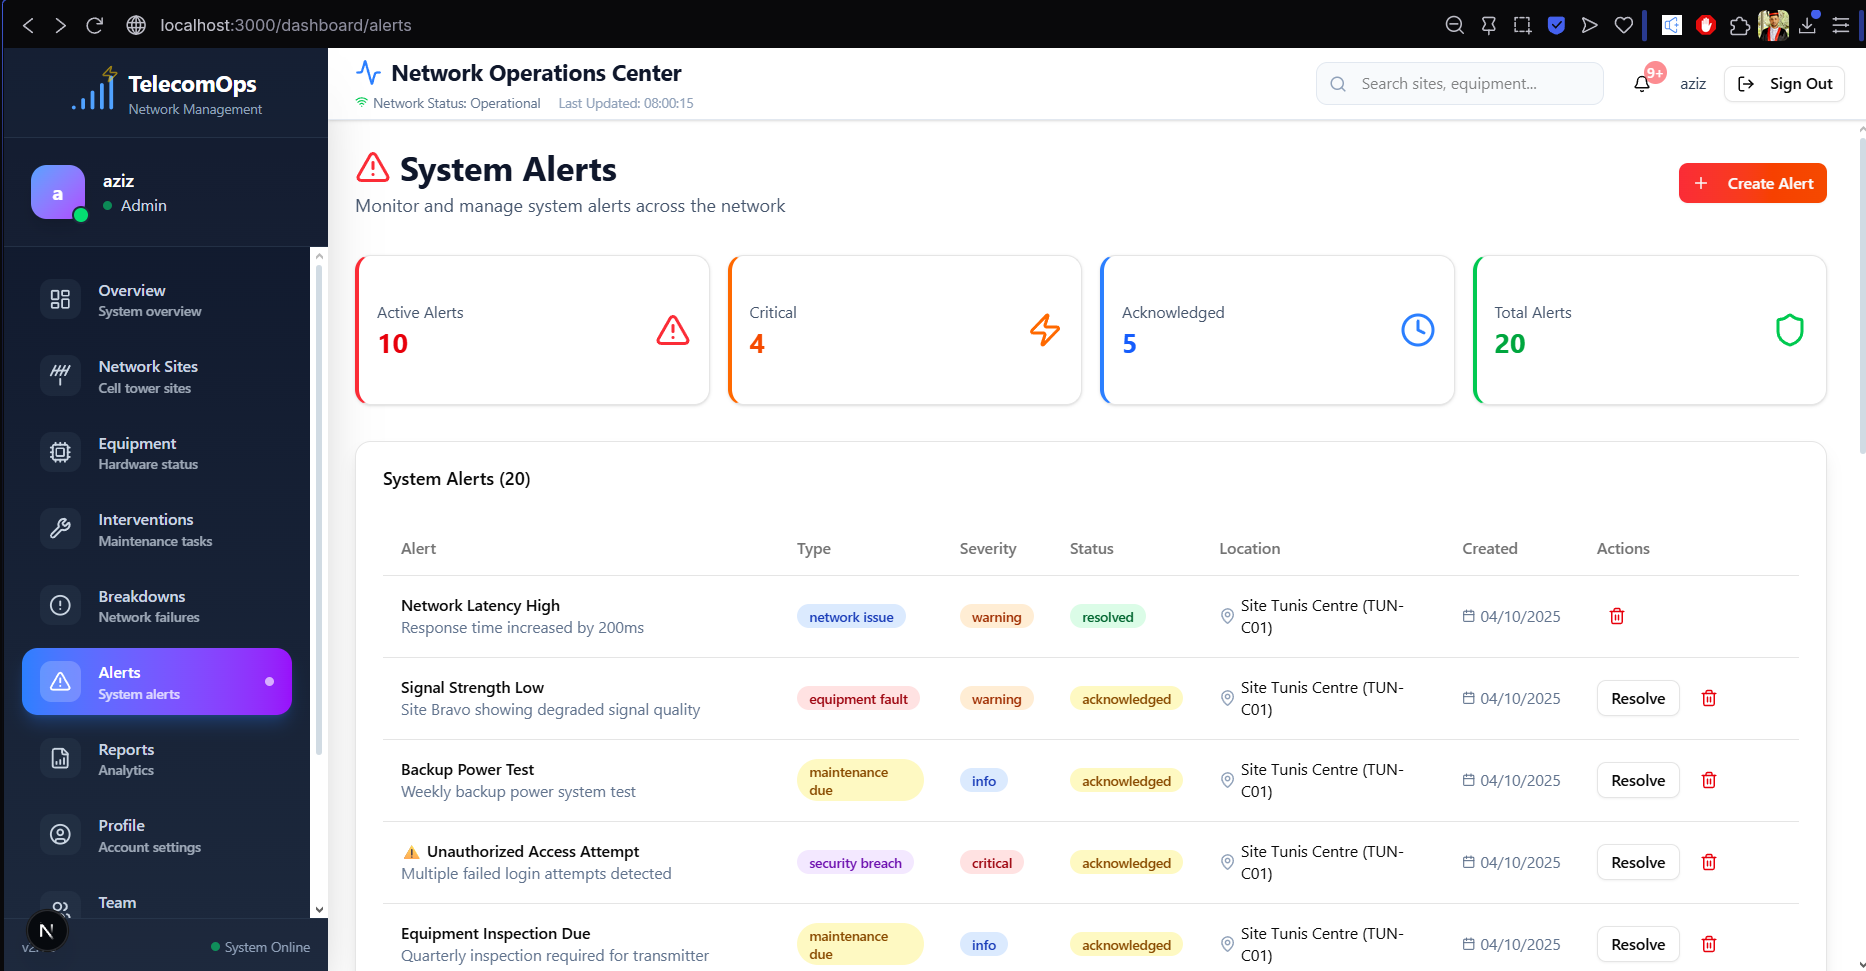
\includegraphics[width=0.9\linewidth]{img/chap_06/screenshot_alerts_dashboard.png}
    \caption{Alert Management Dashboard with Statistics}
    \label{fig:alerts_dashboard}
\end{figure}

The alert dashboard (Figure 6.5) displays statistics showing active alerts, critical alerts, acknowledged alerts, and total alert count. The alerts table presents detailed information with columns for alert title, type badge, severity level with visual indicators, current status, site location, creation timestamp, and role-appropriate action buttons. The interface supports real-time updates with new alerts appearing automatically.

\subsection{Create Alert Form}

Figure 6.6 presents the alert creation form enabling manual alert generation with comprehensive validation.

\begin{figure}[H]
    \centering
    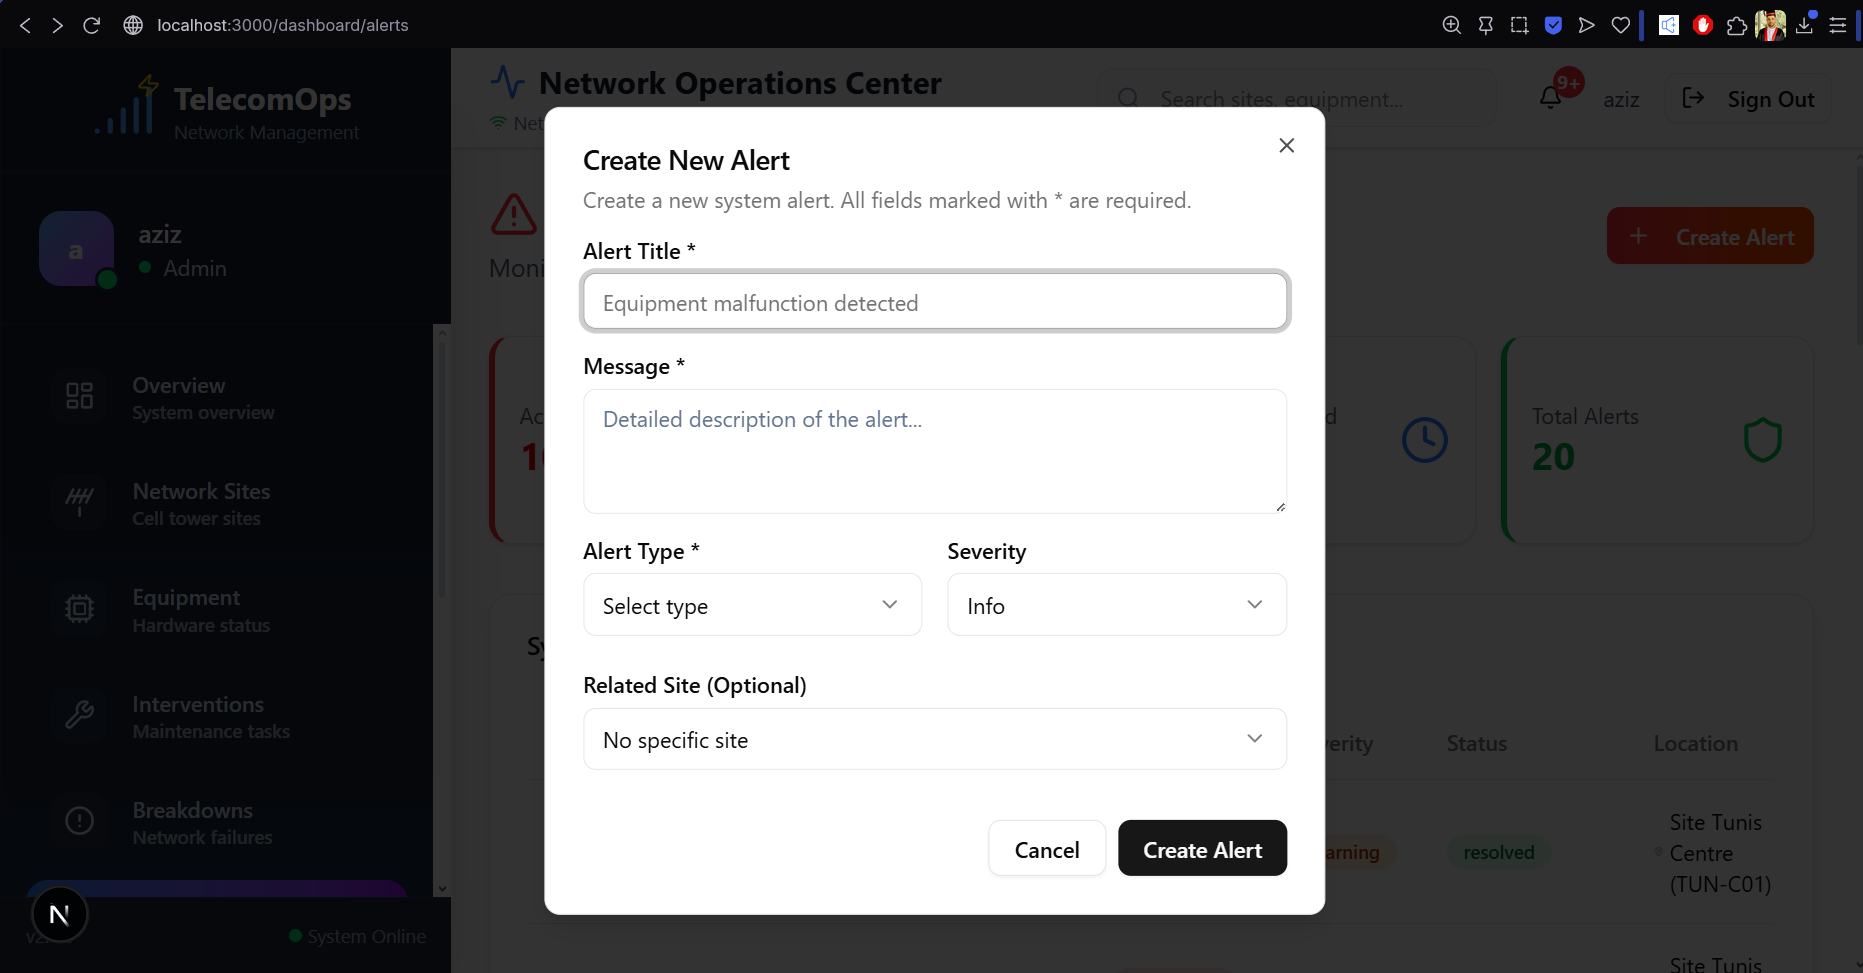
\includegraphics[width=0.7\linewidth]{img/chap_06/screenshot_create_alert.png}
    \caption{Create Alert Form with Validation}
    \label{fig:create_alert_form}
\end{figure}

The alert creation form (Figure 6.6) includes required fields for alert title, detailed message textarea, alert type dropdown with predefined categories, severity level selection with color-coded indicators, site dropdown with search functionality, and optional equipment dropdown loading dynamically based on selected site. The form implements comprehensive validation ensuring title length between 5-100 characters and required selections for type and severity.

\subsection{Real-time Alert Notification}

Figure 6.7 illustrates the real-time notification toast appearing when critical alerts are created.

\begin{figure}[H]
    \centering
    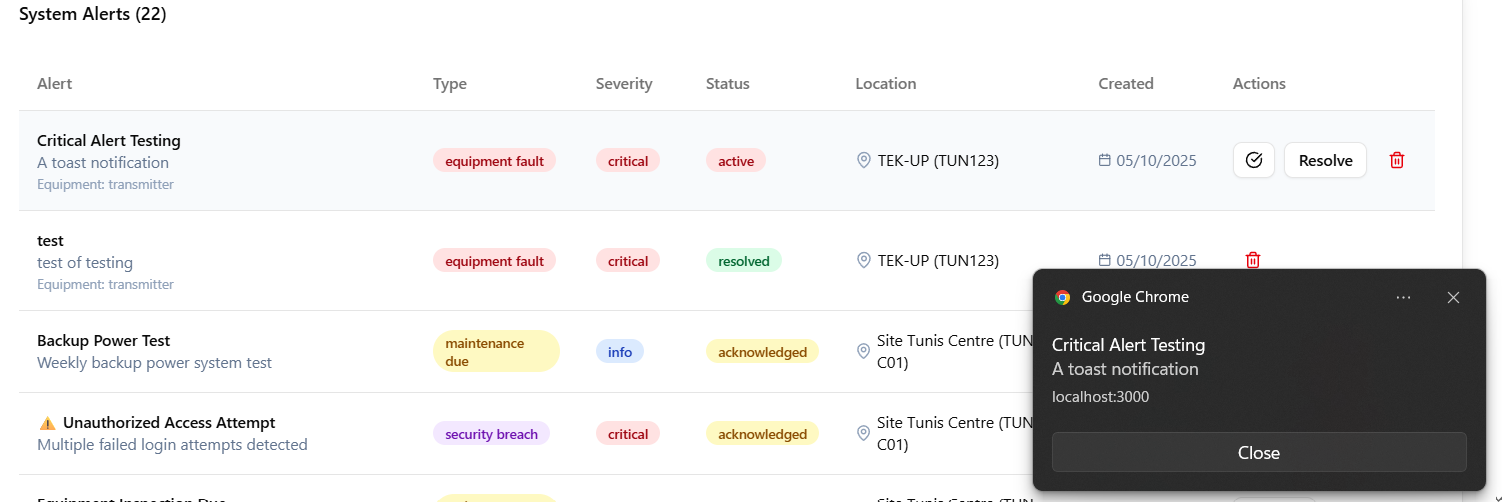
\includegraphics[width=1\linewidth]{img/chap_06/screenshot_alert_toast.png}
    \caption{Real-time Alert Notification Toast}
    \label{fig:alert_notification}
\end{figure}

The notification toast (Figure 6.7) appears in bottom-right corner with slide-in animation, displays alert icon with severity-based color, shows alert title and brief description, indicates creation timestamp, provides action buttons for immediate acknowledgment or viewing details, includes dismiss button for manual closure, and auto-dismisses after 10 seconds if not interacted with. Multiple notifications stack vertically with proper spacing.

\subsection{Alert Details View}

Figure 6.8 presents the detailed alert view showing complete information and status history.

\begin{figure}[H]
    \centering
    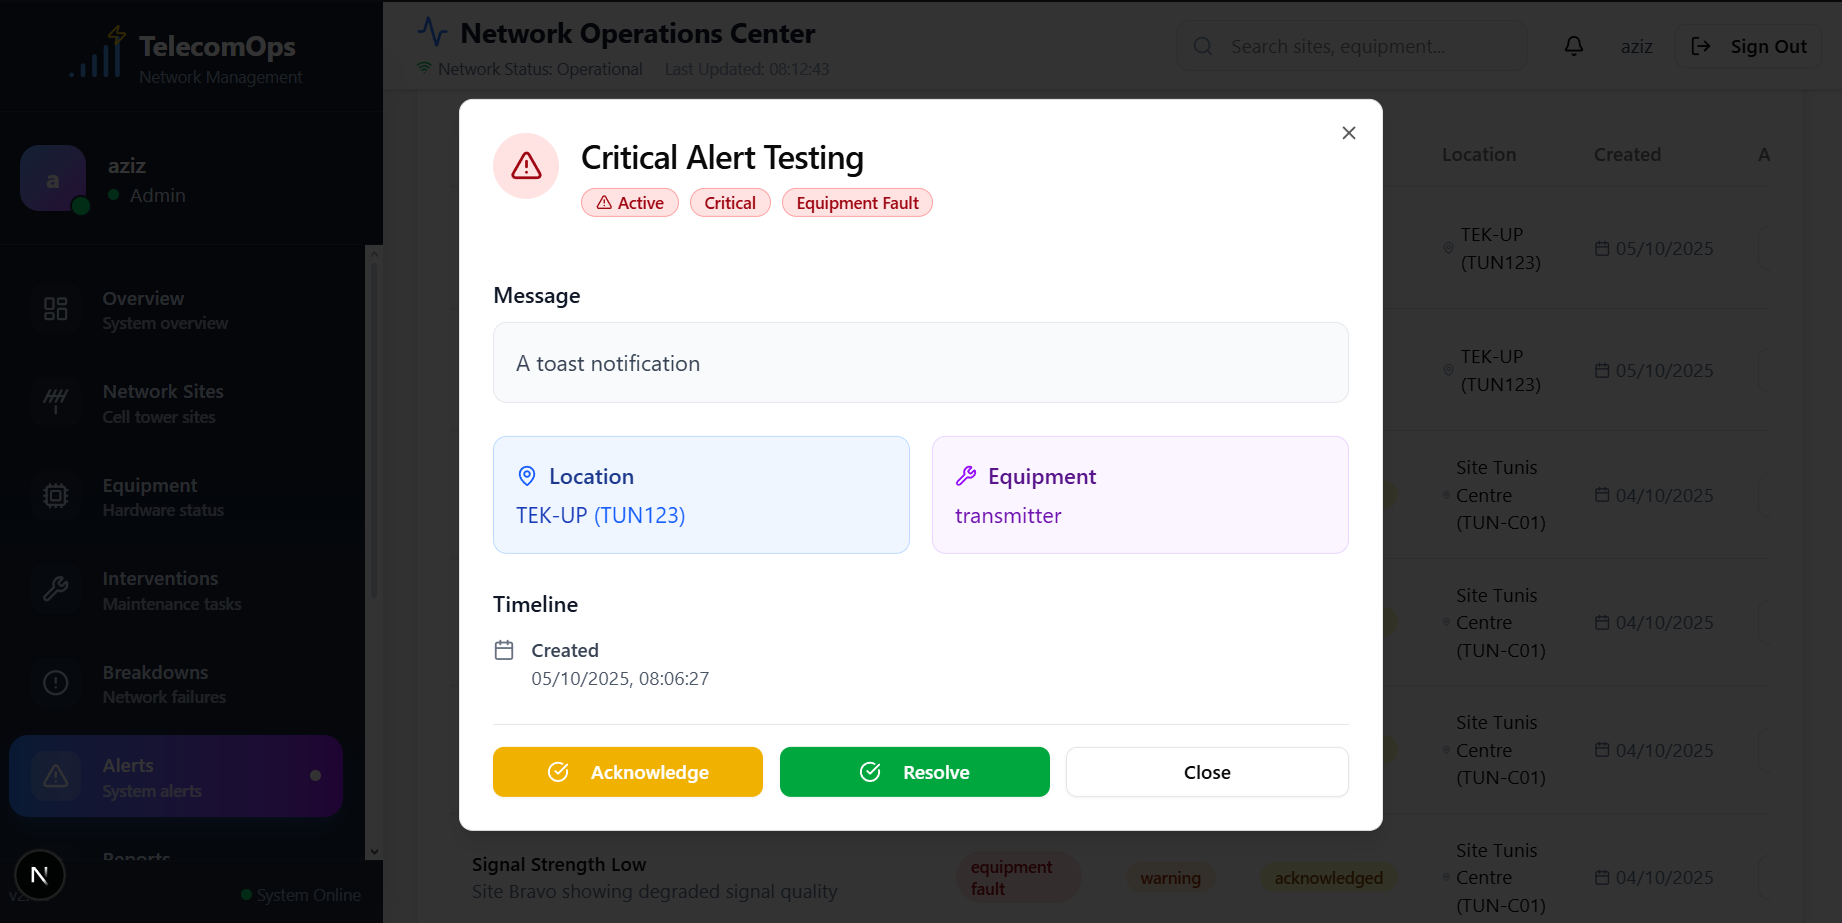
\includegraphics[width=0.85\linewidth]{img/chap_06/screenshot_alert_details.png}
    \caption{Alert Details with Status History}
    \label{fig:alert_details}
\end{figure}

The alert details view (Figure 6.8) displays complete alert information including full title and message, type and severity with visual indicators, current status with workflow position, associated site and equipment with hyperlinks, creation timestamp with relative time display, acknowledgment timestamp if acknowledged, resolution timestamp if resolved, response time calculation for performance metrics, and action buttons appropriate to current status and user role.

\subsection{Energy Consumption Dashboard}

Figure 6.9 illustrates the energy consumption dashboard with statistics and trend visualization.

\begin{figure}[H]
    \centering
    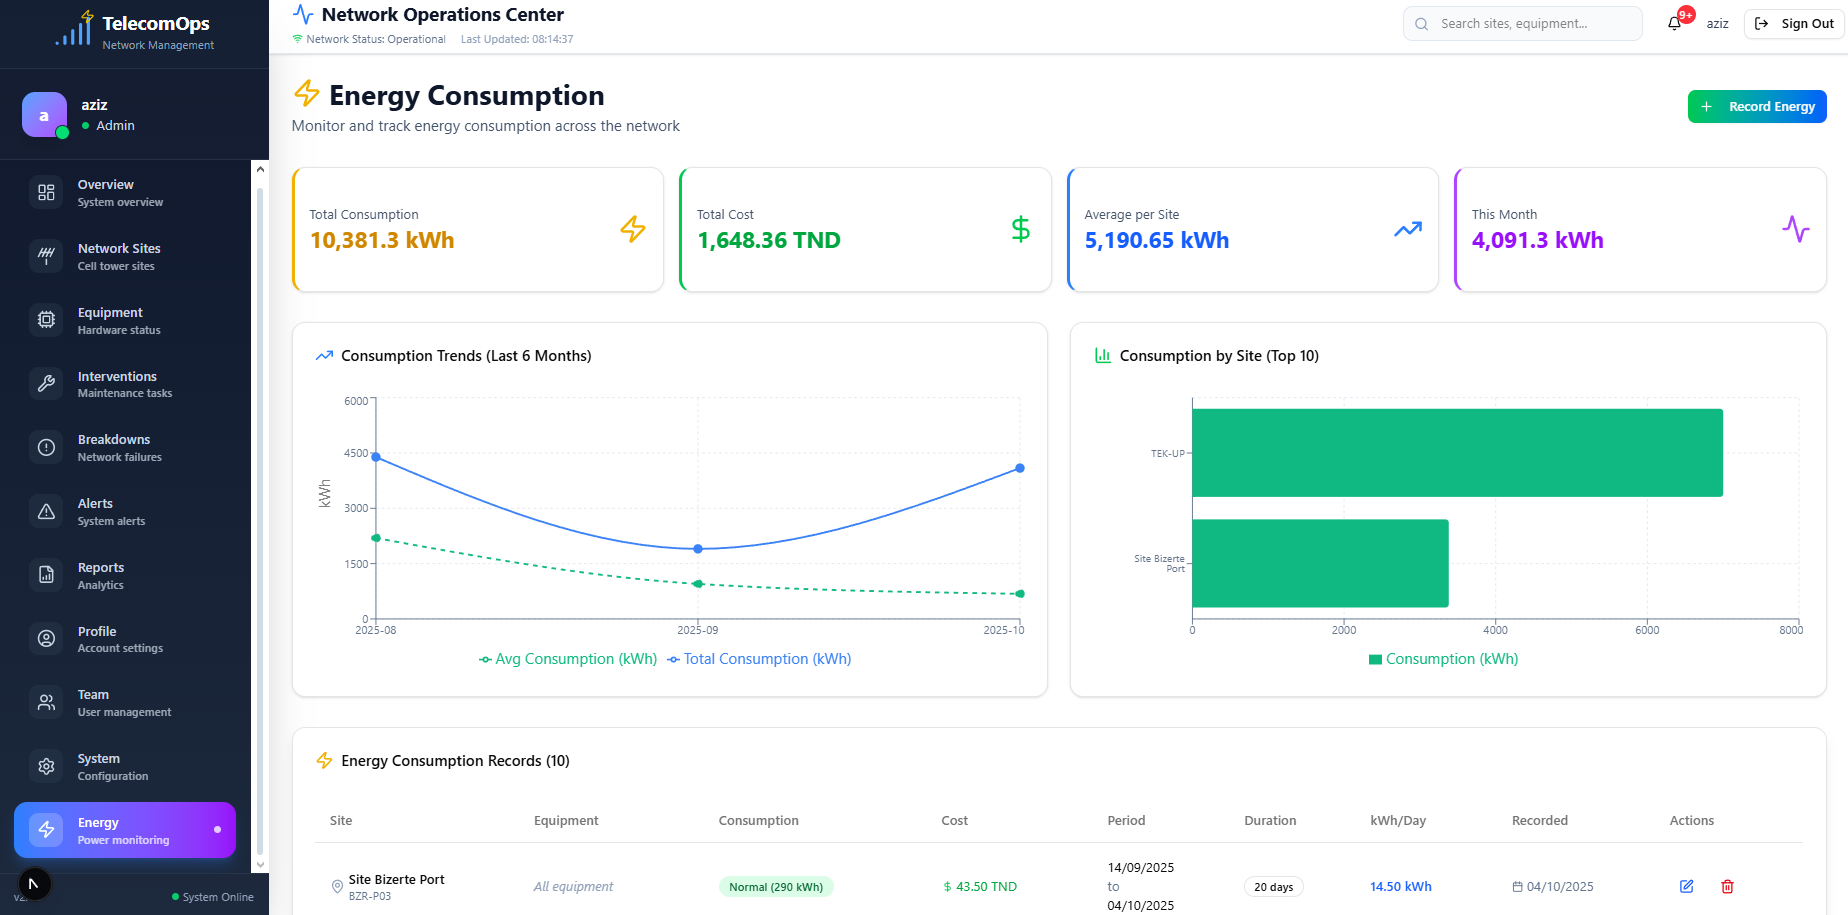
\includegraphics[width=0.9\linewidth]{img/chap_06/screenshot_energy_dashboard.png}
    \caption{Energy Consumption Dashboard with Charts}
    \label{fig:energy_dashboard}
\end{figure}

The energy dashboard (Figure 6.9) displays comprehensive statistics showing total consumption in kWh for selected period, total cost in Tunisian Dinars, average daily consumption, and monthly trend indicator. The dashboard features interactive charts showing 6-month consumption trend with line graph, bar chart comparing top 10 sites by consumption, and period selector for custom date ranges. Color coding indicates consumption levels: green for normal, orange for elevated, red for excessive.

\subsection{Record Energy Form}

Figure 6.10 presents the energy consumption recording form with automatic cost calculation.

\begin{figure}[H]
    \centering
    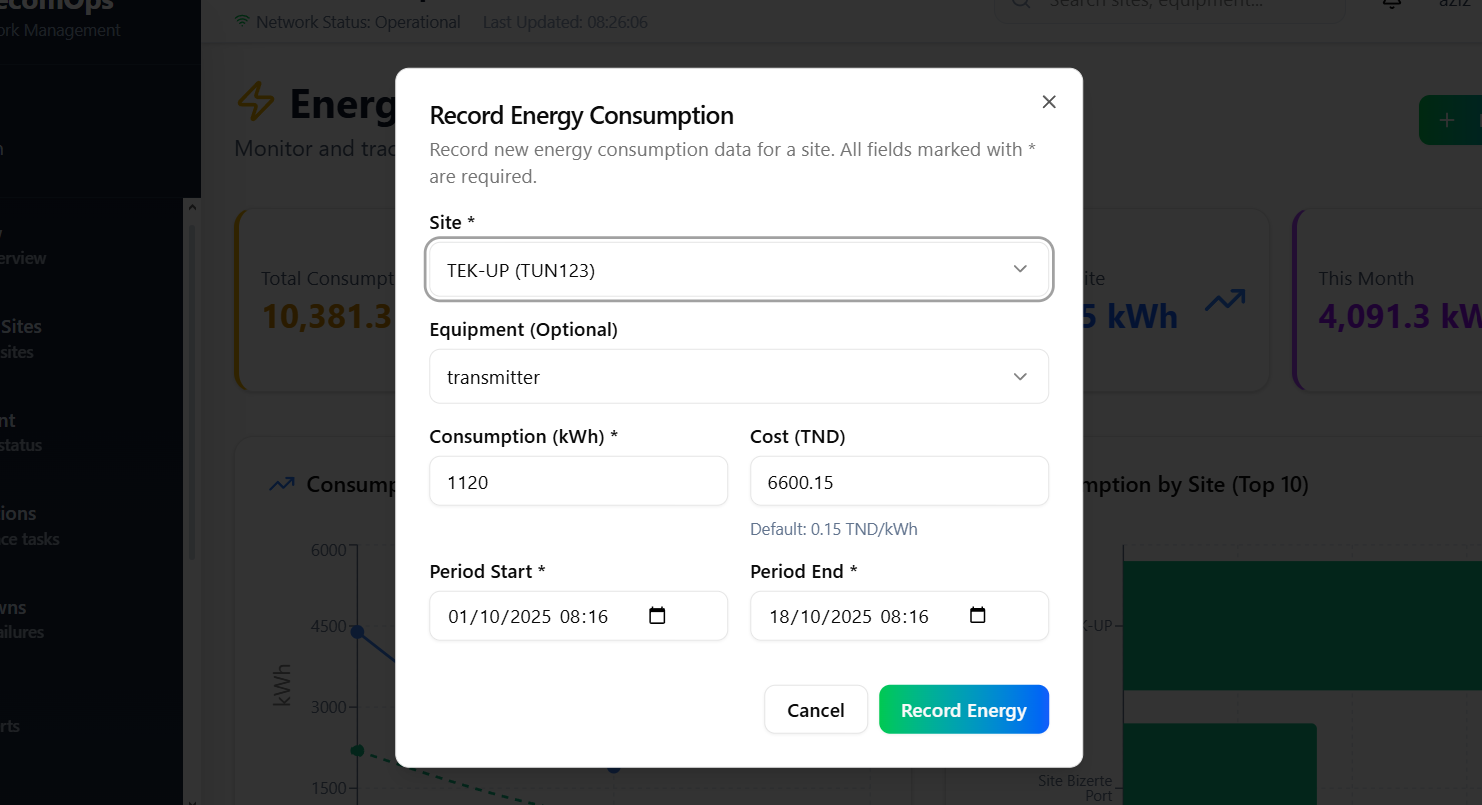
\includegraphics[width=0.7\linewidth]{img/chap_06/screenshot_record_energy.png}
    \caption{Record Energy Consumption Form}
    \label{fig:record_energy_form}
\end{figure}

The energy recording form (Figure 6.10) includes site dropdown with search capability, optional equipment selection for asset-specific tracking, consumption input field accepting decimal values in kWh, recording period with start and end date pickers, automatic cost calculation displaying calculated cost at 0.15 TND/kWh, optional manual cost override field, and submission button with validation feedback. Real-time calculation updates cost as user enters consumption value.

\subsection{Energy Consumption Table}

Figure 6.11 illustrates the consumption records table with color-coded values and filtering.

\begin{figure}[H]
    \centering
    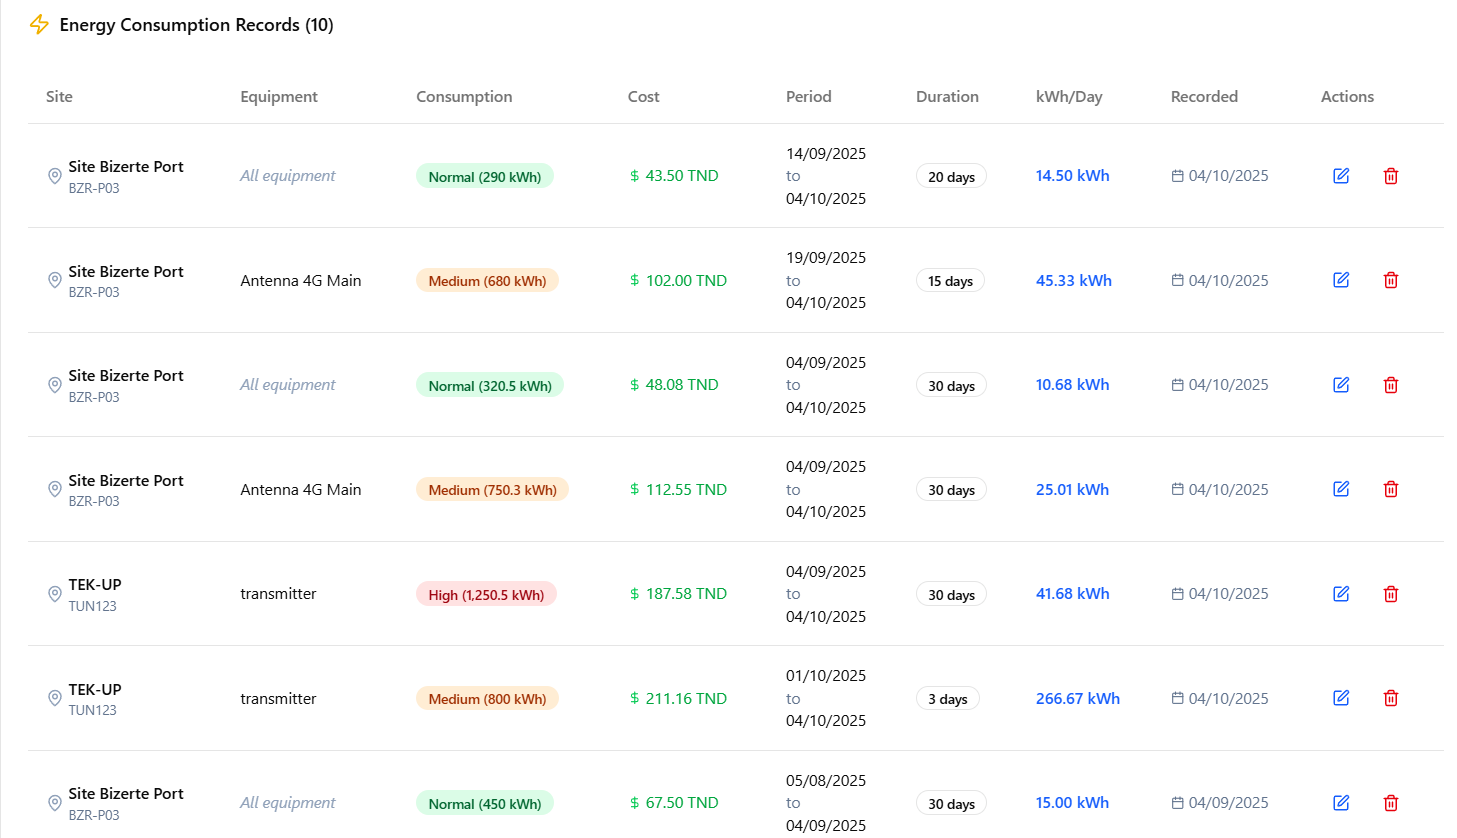
\includegraphics[width=0.9\linewidth]{img/chap_06/screenshot_energy_table.png}
    \caption{Energy Consumption Records Table}
    \label{fig:energy_table}
\end{figure}

The consumption table (Figure 6.11) displays site name with location, equipment if specified, consumption value with color coding (red >1000 kWh, orange 500-1000 kWh, green <500 kWh), calculated cost in TND, recording period with duration calculation, daily consumption rate, recording timestamp, and action buttons for viewing details and editing records with appropriate permissions.

\subsection{Consumption Trend Charts}

Figure 6.12 presents the interactive consumption trend charts with multi-period analysis.

\begin{figure}[H]
    \centering
    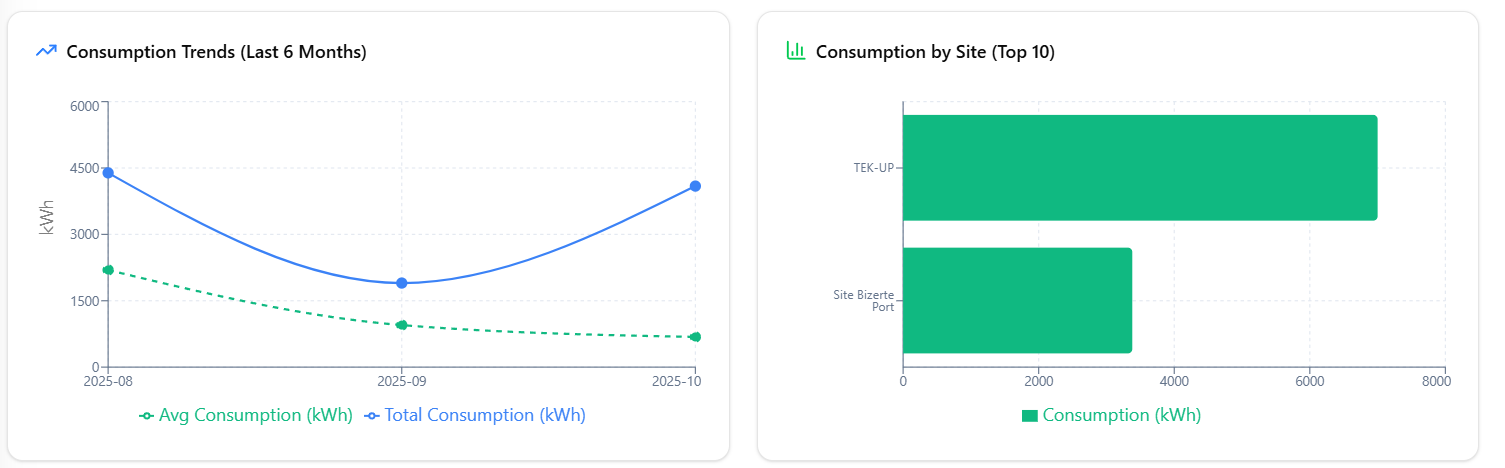
\includegraphics[width=0.9\linewidth]{img/chap_06/screenshot_energy_charts.png}
    \caption{Energy Consumption Trend Analysis}
    \label{fig:energy_charts}
\end{figure}

The charts (Figure 6.12) display 6-month consumption trend with line graph showing monthly totals, bar chart comparing top 10 highest-consuming sites, pie chart showing consumption distribution by region, and interactive tooltips displaying exact values on hover. Period selector enables custom date range analysis with preset options for last week, month, quarter, and year.

\section{Technical Challenges and Solutions}

Sprint 4 implementation encountered several technical challenges requiring sophisticated solutions.

\subsection{Real-time Alert Notification Architecture}

\textbf{Challenge:} Implementing scalable real-time notifications with minimal latency across distributed user sessions. The system required sub-200ms notification delivery while supporting hundreds of concurrent users and maintaining connection stability.

\textbf{Solution:} The solution leverages Supabase WebSocket subscriptions providing bidirectional real-time communication. The Real-time Engine maintains persistent WebSocket connections with automatic reconnection logic implementing exponential backoff strategy. Critical alerts broadcast events to subscribed clients through Supabase channels enabling targeted delivery based on user roles.

The AlertNotificationToast component implements reconnection logic with exponential backoff, queues messages during disconnection, and implements message deduplication. Server-side event filtering reduces bandwidth by sending alerts only to relevant users. Connection pooling supports thousands of concurrent connections while maintaining sub-200ms delivery latency.

\subsection{Energy Cost Calculation Flexibility}

\textbf{Challenge:} Implementing flexible cost calculation supporting both automatic rate-based calculation and manual cost overrides for varying pricing models and special billing scenarios.

\textbf{Solution:} The Cost Calculator component implements dual-mode calculation logic. In automatic mode, the system multiplies consumption by configured rate (0.15 TND/kWh), displays calculated cost in real-time, and stores calculated cost with automatic flag. In manual override mode, users can enter custom cost value. The system stores override flag indicating manual calculation and displays indicator showing cost was manually specified.

Client-side calculation provides immediate feedback, while server-side calculation ensures data integrity. Centralized rate configuration accessible only to administrators ensures consistent application. Historical records remain unchanged when rates update.

\subsection{Consumption Analytics Aggregation Performance}

\textbf{Challenge:} Efficiently aggregating large consumption datasets comprising thousands of records while providing real-time analytics dashboards with sub-second response times.

\textbf{Solution:} The solution implements multi-layered aggregation using PostgreSQL materialized views, in-memory caching, and optimized query patterns. Materialized views pre-compute monthly and daily aggregations with incremental refresh. Dashboard queries access materialized views instead of raw records, reducing query execution time from seconds to milliseconds.

SQL window functions enable efficient trend calculations and comparative analysis. React Query caching stores aggregated results with 5-minute TTL. Redis caching provides sub-100ms response times for high-traffic queries. Chart rendering optimization includes data point reduction for large datasets and lazy loading for components.

\section{Testing and Validation}

Sprint 4 underwent comprehensive testing ensuring reliability, real-time functionality, and proper integration.

\subsection{Functional Testing}

Alert functional testing validated complete CRUD operations, form submission with all field combinations, type and severity selection, site and equipment association, status transitions through workflow, user tracking, and timestamp accuracy. Notification testing verified real-time delivery within 200ms, toast component rendering with animations, auto-dismiss after 10 seconds, manual dismiss capability, multiple notification stacking, and persistence across page refreshes.

Energy functional testing validated numeric input with decimal precision, automatic cost calculation accuracy, manual cost override functionality, date validation, equipment association handling, threshold violation detection, and automatic alert generation. Chart testing confirmed data accuracy matching source records, aggregation correctness for all time periods, proper axis scaling, interactive tooltip functionality, and responsive design across screen sizes.

\subsection{Integration Testing}

Database integration testing verified Supabase connectivity, Row Level Security enforcement for all operations, foreign key constraint integrity, and transaction integrity ensuring atomic operations. Real-time integration testing confirmed WebSocket connection establishment, event broadcasting to all subscribed clients, automatic reconnection after interruptions, message ordering preservation, and proper connection cleanup on logout.

Authentication integration testing validated role-based access control for all operations, JWT token validation, session management across multiple tabs, and unauthorized access prevention. Form integration testing verified cascading dropdown population, validation consistency between client and server, error message propagation, and optimistic UI updates with automatic rollback on errors.

\subsection{Performance Testing}

Alert performance validation confirmed creation operations complete within 300ms, notification delivery averages 150ms, dashboard loading displays 1000+ alerts in under 2 seconds, and system supports 100+ concurrent users without degradation. Energy performance testing validated calculation accuracy, chart rendering completes in under 1 second for 1000+ data points, aggregation queries execute in under 500ms for 10,000+ records, and export operations optimize memory usage.

Load testing simulated 500 concurrent alert creations, 1000 notifications per minute, 10,000 concurrent energy queries, and 1000 database operations per second. Results demonstrate linear scaling to 1000 concurrent users with less than 5% performance degradation.

\subsection{User Acceptance Testing}

Tunisia Telecom operational staff performed user acceptance testing with realistic scenarios. Managers tested alert acknowledgment workflows and validated energy data entry appreciating automatic cost calculation. Engineers tested alert creation with technical descriptions, validated consumption trend analysis charts, and confirmed threshold configuration.

Technicians tested mobile alert notifications and validated energy recording from field locations. Administrators tested system configuration including alert rules and threshold management, validated permission enforcement, and confirmed audit trail completeness. Overall feedback was positive with users appreciating real-time responsiveness, intuitive visualizations, and automatic calculations.

\section{Sprint Review and Retrospective}

Sprint 4 review with stakeholders confirmed successful delivery of all committed user stories addressing US-010, US-011A, and US-011B from Chapter 2's product backlog. Stakeholders particularly valued the real-time notification system, automatic cost calculation, comprehensive trend visualizations, and threshold-based alerting.

The sprint retrospective identified positive outcomes including Supabase real-time subscriptions providing reliable infrastructure, PostgreSQL materialized views delivering exceptional query performance, React Query caching reducing server load, and comprehensive validation preventing data quality issues. Areas for improvement identified include earlier performance testing with production-scale data, additional mobile device testing, enhanced documentation for troubleshooting, and more comprehensive error handling for edge cases.

\section{Conclusion}

Sprint 4 successfully delivered comprehensive alert management and energy consumption monitoring capabilities significantly enhancing TelecomOps operational effectiveness. The implementation addressed all committed user stories from Chapter 2's product backlog, providing complete real-time notification infrastructure and comprehensive energy tracking capabilities.

The Alert Management System enables proactive incident response through automated alert generation from equipment status changes established in Sprint 2, manual alert creation for observed issues, intelligent severity classification, workflow-based status management, and real-time notification delivery achieving sub-200ms latency. The system supports both automated and manual alert creation, maintains complete audit trails, and integrates seamlessly with existing site and equipment management from Sprints 1 and 2.

The Energy Consumption Monitoring System enables data-driven energy management through comprehensive consumption recording, automatic cost calculation using configurable rates, visual analytics through interactive charts, threshold-based alerting for abnormal patterns, and efficient aggregation processing thousands of records. The system supports both site-level and equipment-level tracking, maintains historical data integrity, and provides actionable insights through comparative analysis.

Technical achievements demonstrate production-ready architecture with real-time WebSocket infrastructure supporting 1000+ concurrent users, flexible cost calculation, high-performance analytics using PostgreSQL materialized views, responsive user interfaces, and comprehensive validation. Performance metrics exceed Chapter 2's non-functional requirements with dashboard load times under 2 seconds, notification delivery under 200ms, and linear scaling to 1000 concurrent users.

The implementation establishes foundation for advanced operational capabilities including machine learning-based anomaly detection, predictive alerting, automated resolution recommendations, comparative site analytics, consumption forecasting, and external system integration supporting organizational sustainability goals. Quality metrics exceeded established targets with successful stakeholder validation, performance exceeding NFR-001 requirements, comprehensive test coverage, and positive user feedback.

The next chapter presents Sprint 5, introducing advanced features including predictive maintenance using historical breakdown and intervention data from Sprint 3, comprehensive reporting and analytics dashboards, and system administration capabilities, completing the core TelecomOps platform functionality.